%%%%%%%%%%%%%%%%%%%%%%%%%%%%%%%%%%%%%%%%%%%%%%%%%%%%%%%%%%%%%%%%
% Sablona pro zaverecnou zpravu k semestralni praci z BI-ZUM
% Kódování dokumentu: UTF8
% Verze: 1.0 (2013-01-28)
% Autor: Ing. Martin Šlapák
%%%%%%%%%%%%%%%%%%%%%%%%%%%%%%%%%%%%%%%%%%%%%%%%%%%%%%%%%%%%%%%%
%
% NEUPRAVUJTE PROSIM PARAMETRY DOKUMENTU, JAKO OKRAJE CI PISMO!
%
%%%%%%%%%%%%%%%%%%%%%%%%%%%%%%%%%%%%%%%%%%%%%%%%%%%%%%%%%%%%%%%%
%
% Celkova delka zpravy nesmi presahnout 1 stranu A4, vyjadrujte 
% se strucne, jasne a vecne - zadne omacky a slovni vata. Diky!
% Neprehazujte ani poradi sekci.
%
%%%%%%%%%%%%%%%%%%%%%%%%%%%%%%%%%%%%%%%%%%%%%%%%%%%%%%%%%%%%%%%%
\documentclass[a4paper,10pt,twocolumn]{article}
\usepackage{lmodern}
\usepackage[czech]{babel}
\usepackage[T1]{fontenc}
\usepackage[utf8]{inputenc}
\usepackage{graphicx}
\usepackage{float}
\usepackage[top=0.5cm,bottom=2cm,left=1cm,right=1cm]{geometry}
%gobble sezere cisla stranek, takze nebudou zadna
\pagenumbering{gobble} 
\title{Zpráva k 5. domácímu úkolu z předmětu MI-PAA}
\date{\today}
%%%%%%%%%%%%%%%%%%%%%%%%%%%%%%%%%%%%%%%%%%%%%%%%%%%%%%%%%%%%%%%%
% tady nastavte své jméno a email
\author{Jan Sokol \\ sokolja2@fit.cvut.cz}
%%%%%%%%%%%%%%%%%%%%%%%%%%%%%%%%%%%%%%%%%%%%%%%%%%%%%%%%%%%%%%%%
\begin{document}
\maketitle
%%%%%%%%%%%%%%%%%%%%%%%%%%%%%%%%%%%%%%%%%%%%%%%%%%%%%%%%%%%%%%%%
\begin{abstract}

Je dána booleovská formule $F$ proměnnných $X=(x_1, x_2, ... , x_n)$ v konjunktivní normální formě (tj. součin součtů). Dále jsou dány celočíselné kladné váhy $W=(w_1, w_2, ... , w_n)$. Najděte ohodnocení $Y=(y_1, y_2, ... , y_n)$ proměnných $x_1, x_2, ... , x_n$ tak, aby $F(Y)=1$ a součet vah proměnných, které jsou ohodnoceny jedničkou, byl maximální. \\

Je přípustné se omezit na formule, v nichž má každá klauzule právě 3 literály (problém $3 SAT$). Takto omezený problém je stejně těžký, ale možná se lépe programuje a lépe se posuzuje obtížnost instance (viz Selmanova prezentace v odkazech).\\
Obdobný problém, který má optimalizační kritérium ve tvaru "aby počet splněných klausulí byl maximální" a kde váhy se týkají klausulí, se také nazývá problém vážené splnitelnosti booleovské formule. Tento problém je lehčí a lépe aproximovatelný. Oba problémy se často zaměňují i v seriózní literatuře.

% Zde shrňte v několika větách co jste dělali, jak jste to dělali, jakých výsledků jste dosáhli. Vypíchněte to nejzajímavější. Zkusili jste nějakou pokročilou techniku? Tady se s ní pochlubte a pak ji dále rozepište v patřičné sekci. Zkuste se vejít do 150 slov.
\end{abstract}

%%%%%%%%%%%%%%%%%%%%%%%%%%%%%%%%%%%%%%%%%%%%%%%%%%%%%%%%%%%%%%%%

\section{Úvod do problému}

SAT je problém splnitelnosti. V logice vyjadřuje problém odpověd na otázku, zdali existuje zadanému výrazu (formuli) zapsaného ve výrokové Booleovské logice pomocí operací AND, OR a NOT přiřazení, při kterém bude výraz ohodnocen jako pravdivý.

$$
x_1\land x_2\land x_3
$$

Problém nazývaný "3SAT", "3CNFSAT", nebo "3-satisfiability" je definování speciálního případu, kdy určení splnitelnosti formule v konjunktivní normální formě, kde každá klauzule je omezena na nejvýše tři literály.

$$
(x_1\lor x_2\lor x_3)\land (x_5\lor x_6\lor x7)
$$


MAX-SAT problem je generalizace SAT problému. Je to problém určení maximálního počtu klauzulí, dané formule, které můžou být splnitelné pro nějaké přiřazení hodnot.

Vážený (Weighted) MAX-SAT se ptá, jaká může být maximální váha splnitelná pro všechny přiřazení, s tím že máme dány vážené hodnoty klauzulí.

\section{Vstupní formát dat - DIMACS}

Všechny testovací úlohy byly získány modifikací1 příslušných úloh z DIMACS formátu. 

Formát DIMACS slouží pro standardizovanou reprezentaci logické formule pro řešení SAT problému. Pomocí DIMACS  jsou definovány dva různé formáty uložení. První slouží pro reprezentaci  formule v konjunktivní normální formě, a je označován jako DIMACS CNF. Druhý  formát  slouží  pro  reprezentaci  obecné  logické  formule a je označován jako SAT - my budeme vycházet z toho prvního.

Formát je oproti originálnímu DIMACS CNF formátu poněkud upraven a vypadá takto:
   \begin{verbatim}
c cnf with weights
p cnf 6 4
w 2 4 6 8 4 2
1 2 -3 0
-2 4 0
1 4 5 6 0
   \end{verbatim}

Díky tomu jsou do CNF přidány též váhy jednotlivých proměnných. Tyto hodnoty jsou obsaženy na řádku (začínajícím s w) pod definicí problému (začínajícím s p).


Z prezentace Stochastic Search And Phase Transitions: AI Meets Physics víme, že nejtěžší  3SAT problémy mají poměr 4.3 (poměr klauzulí ku počtu proměnných). Na tyto instance se budeme nejvíce zaměřovat.


Všechny zvolené instance dat, které budou měřena, jsou s 20-ti proměnnými, liší se v počtu klauzulí, konkrétně je to 45, 70 a 91. V závěru práce se pak pokusím spustit algoritmus i na těžší varianty s větším počtem proměnných - instance s 218 klauzulemi a 50 proměnnými (odpovídá poměru 4.36, tedy nejtěžší problémy).

% The problem of determining the maximum number of clauses, of a given Boolean formula, that can be satisfied by some assignment.

% Weighted MAX-SAT asks for the maximum weight which can be satisfied by any assignment, given a set of weighted clauses.

% Here is weighted 3-SAT problem going to be investigated.


\section{Práce s omezujícími podmínkami}

Největším rozdílem od problému batohu zde jsou přísné omezující podmínky, které prostor dělají přetržitým a hůře dostupným.

Proto jsem musel omezující podmínky relaxovat. Do dalších generací procházejí i ti jedinci, kteří podmínky porušují. Až v poslední generaci jsou vybráni ti nejlepší jedinci, kteří podmínky splňují.

\section{Cenová (fitness) funkce}

Když porovnáváme 2 stavy ze stavového prostoru úlohy, potřebujeme funkci, která umí jednotlivé stavy kvalitativně ocenit. Na rozdíl od problému batohu si však u váženého 3 SATu nevystačíme s pouhým porovnáním dosažené váhy. Musíme ale v zřetel brát i podmínku splnitelnosti formule. Navržena byla proto následující cenová funkce:
$$
h(X) = ln(k \cdot e^{\frac{C_X}{C_{total}}} - (1 - k) \cdot e^{\frac{W_X}{W_{total}}}})
$$

\\
kde $C_X$ je počet splněných klauzulí stavu $X$, $C_{total}$ počet klauzulí formule F, $W_X$ váha stavu X a $W_{total}$ suma vah všech proměnných formule F.

k je zde koeficient chtěné vlastnosti. Pro hodnotu 0 preferujeme pouze co nejvyšší součet vah, pro hodnotu 1 bychom preferovali pouze co nejvíce splněných klauzulí.


Pozn. v grafech níže je výsledek fitness funkce vynásoben tisícem, pro lepší zobrazení v grafech.
% Cílem je zvolit tuto hodnotu k co nejrozumněji. Hodnota musí být vyšší, než 0.5, jelikož chceme vyjádřit penalizaci za nesprávné řešení, ale zároveň musí být nižší, než 1, jinak bychom součty vah ignorovali a hledali jen splnitelnost.

\section{Výběr jazyka}
Pro svou implementaci problému batohu jsem si vybral jazyk Python. Ačkoli to je jazyk interpretovaný a nečekal jsem závratné rychlosti výpočtů, mojím výběrem byl pro to, že jsem jazyk znal a pro jakýkolik koncept je pro mne nejrychlejší.


\section{Testovací Hardware}
Všechny testy byly prováděny na cloudové linuxové instanci v AWS, běžící na Red Hat Enterprise Linux 7. Velikost instance byla:
  2 Core CPU / 8 GB RAM, v názvosloví AWS \textbf{m4.large}.


\section{Měření výpočetního času}
Výpočet běhu funkce je řešen tak, že je spočten strojový čas před během funkce, a také po něm. Tyto časy jsou od sebe odečteny a je vrácen čas v ms.

   \begin{verbatim}
def timing(f):
    def wrap(*args):
        time1 = time.time()
        ret = f(*args)
        time2 = time.time()
        measured_time.append(
          {'type': f.__name__,
           'time': (time2-time1)*1000.0})
        return ret
    return wrap
   \end{verbatim}


\subsection{Popis algoritmu}

Zde uvádím úryvek kódu řídící evoluci. Celý funkční kód je k dispozici v repozitáři.

Nejdříve vytvoříme počáteční populaci. Potom v n generacích běžíme nasledovné:
\begin{itemize}
  \item vytřídíme nejlepší jedince dle fitness funkce necháme je soupeřit v turnaji,
  \item dle nastaveného elitismu převezmeme x jedinců z minulého kola do tohoto,
  \item vyplníme novou generaci novými jedinci, kteří jsou:
\begin{itemize}

  \item kříženci dvou náhodných minulých jedinců,
  \item nebo jeden náhodný jedinec.
\end{verbatim}
  \item mutujeme náhodné bity těchto nových jedinců
  \item ověříme, zda jedinec je validní (náklad batohu je menší, než je jeho kapacita).

\end{verbatim}

   \begin{verbatim}

# Create initial population
population = create_population(self.population_size,
                                    size)

# Run n generations
for generation in range(0, self.generations):
  sorted_population = sort_population(population)

  # Selection
  new_population = self.tournament(population,
                       self.tournament_count, 
                       self.tournament_pool_size )

  # Elitsm
  del sorted_population[self.elitism_count:]

  new_population.extend(sorted_population)
  sorted_population = sort_population(new_population)

  # Fill population with new children
  while len(new_population) != self.population_size:
      child = []
      # Crossover
      if odds_are(self.xover_probability):
          in1 = self.random_individual(new_population)
          in2 = self.random_individual(new_population)

          child = self.crossover_single(in1, in2)
      else:
          # Just pick random individual
          child = deepcopy(random_individual(population))

      # Mutation
      child = self.mutator_random_inverse(child,
                           self.mutation_probability)

      # Check if mutated/crossed individual is valid
      if self.constraint_fn(child):
          new_population.append(child)
   \end{verbatim}


\subsection{Výběr parametrů evoluce}

Evoluční algoritmus v přiloženém kódu lze konfigurovat následujícími parametry:
\begin{itemize}

   \item Velikost populace
   \item Počet generací
   \item Pravděpodobnost křížení
   \item Pravděpodobnost mutace
   \item Velikost turnaje
   \item Elitismus
\end{itemize}




\subsection{Experimenty s nastavením parametrů}


Ze začátku jsem vybral stejné parametry, jako u problému batohu. S tím, že mám na paměti, že SAT problém může vyžadovat velmi rozdílné nastavení parametrů.


\begin{figure}[H]
  \begin{center}
    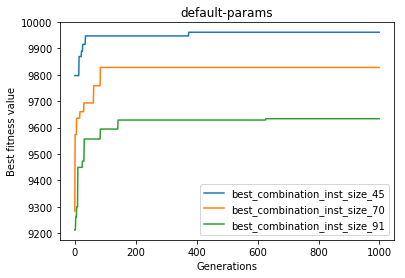
\includegraphics[height=6cm]{graphs/default-params.png}
  \end{center}
  % \caption{Graf vývoje fitness}\label{fig1}
\end{figure}


Tyto výsledky nevypadají vůbec špatně. Například u instance s 45 klauzulemi a 20 proměnnými (té z jednodužších instancí) je výsledná fitness 9961,  což je velmi blízko maximálnímu 10000. Díky tomu můžeme i předpokládat, že se jedná o optimální řešení. 

Na grafech vidíme, že řešení konvergují velmi rychle - kvůli tomu existuje možnost, že můžeme se zaseknout v lokálním maximu.

45-default-params: \\
\begin{tabular}{lrrrrrl}
\toprule
       price &  variables &  clausules &  satisfied &  weight &  valid \\
\hline

\midrule
 9961 &         20 &         45 &         45 &     925 &   True \\
\bottomrule
\end{tabular}
\\


70-default-params: \\
\begin{tabular}{lrrrrrl}
\toprule
       price &  variables &  clausules &  satisfied &  weight &  valid \\
\midrule
\hline

9828 &         20 &         70 &         70 &     783 &   True \\
\bottomrule
\end{tabular}



\\



91-default-params: \\
\begin{tabular}{lrrrrrl}
\toprule
    price &  variables &  clausules &  satisfied &  weight &  valid \\
\midrule
\hline

 9633 &         20 &         91 &         91 &     534 &   True \\
\bottomrule
\end{tabular}


Jak vidíme, tak i kvalita je dobrá. U všech instancí se povedlo nalézt řešení.

% Různě jsem nastavoval parametry genetického algoritmu - pravděpodobnost křížení, pravděpodobnost mutace, elitismus, velikost turnaje, počet turnajů a počet generací. Z grafů jsem poté usoudil, které hodnoty jednotlivých parametrů jsou nejlepší.


\subsection{Náhodnost}

Chceme ověřit, zda náhodnost ovlivňuje výsledky řešení algoritmu. Proto instanci spustíme v 10 bězích a výsledky porovnáme.


\begin{figure}[H]
  \begin{center}
    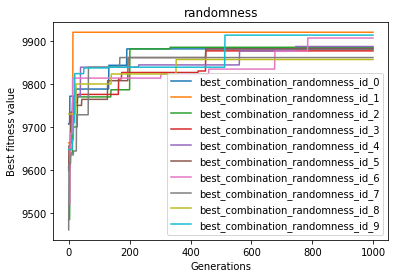
\includegraphics[height=6cm]{graphs/randomness.png}
  \end{center}
  % \caption{Graf vývoje fitness}\label{fig1}
\end{figure}


Všechny tyto instance byly splnitelné a nalezly řešení s fitness lepším, než 9800. Díky tomu soudím, že na data se lze spolehnout.

\subsection{Problém rychlé konvergence}


Rychlou konvergenci k lokálnímu maximu lze vyřešit zvýšením pravděpodobnosti mutace, zvětšení velikosti turnaje a redukcí elitismu.

Experimentálně jsem upravoval parametry tímto směrem. Mutace sice může mít za následek zničení cenných potomků, ale zavede nás na jiná místa stavového prostoru. Navíc s takto strmou konvergencí si to do jisté míry můžeme dovolit.

Zvýšil jsem parametr pravděpodobnosti mutace z 0.1 na 0.5, elitimus z dvou jedinců na jednoho, a nastavil velikost turnaje na 6. Konvergence již není tak rychlá, mělo by docházet k širšímu prohledávání stavového prostoru.



\begin{figure}[H]
  \begin{center}
    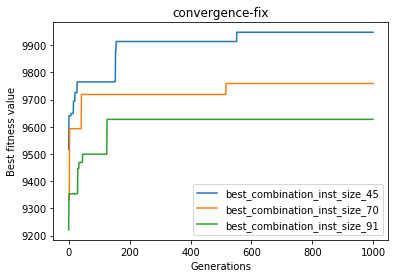
\includegraphics[height=6cm]{graphs/convergence-fix.png}
  \end{center}
  % \caption{Graf vývoje fitness}\label{fig1}
\end{figure}




\\
45-convergence-fix:\\



\begin{tabular}{lrrrrrl}
\toprule
        price &  variables &  clausules &  satisfied &  weight &  valid \\
\midrule
\hline

 9947 &         20 &         45 &         45 &     911 &   True \\
\bottomrule
\end{tabular}
\\



70-convergence-fix:\\



\begin{tabular}{lrrrrrl}
\toprule
        price &  variables &  clausules &  satisfied &  weight &  valid \\
\midrule
\hline

 9758 &         20 &         70 &         70 &     701 &   True \\
\bottomrule
\end{tabular}
\\



91-convergence-fix: \\


\begin{tabular}{lrrrrrl}
\toprule
        price &  variables &  clausules &  satisfied &  weight &  valid \\
\midrule
\hline

 9627 &         20 &         91 &         91 &     524 &   True \\
\bottomrule
\end{tabular}
\\

Jak vidíme tak při této změně jsme schopni nalézt správná řešení i po generaci 600+. Může se také ale velmi často stát, že správné řešení nenalezneme. Tak to dopadá u instance s 91 klauzulemi:

91-convergence-fix:\\
\begin{tabular}{lrrrrrl}
\toprule
        price &  variables &  clausules &  satisfied &  weight &  valid \\
\midrule
\hline

 9628 &         20 &         91 &         90 &     665 &  False \\
\bottomrule
\end{tabular}
\\
\subsection{Pravděpodobnost křížení}
Doporučená pravděpodobnost křížení je 80-95\% (Beasley, 1993). Pomocí selského rozumu také lze usoudit, že malá pravděpodobnost křížení snižuje rychlost konvergence a v případě velmi malé hodnoty vůbec zastaví genetický algoritmus. Avšak pravděpodobnost 100\% taky není dobrá, jelikož ztrácíme rodiče bez jistoty objevu lepšího potomka (algoritmus by měl zachovat "náhodnost" a tím i divergenci populace).

Osobně hodnotím 0.3 až 0.4 jako nejlepší hodnotu pravděpodobnosti křížení. Při pravděpodobnosti 0.7 a více ani nebylo možné dosáhnout optimální hodnoty.

\begin{figure}[H]
  \begin{center}
    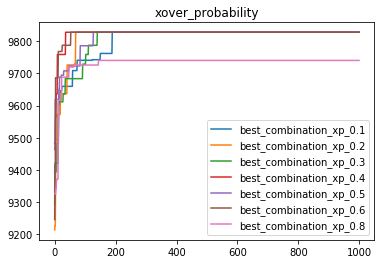
\includegraphics[height=6cm]{graphs/xover_probability.png}
  \end{center}
  % \caption{Graf vývoje fitness}\label{fig1}
\end{figure}

\subsection{Pravděpodobnost mutace}


Na grafu velmi dobře vidíme, že tato hodnota by měla být nízká.
Osobně hodnotím 0.025 až 0.1 jako nejlepší hodnotu pravděpodobnosti mutace. Při pravděpodobnosti 0.7 a více ani nebylo možné dosáhnout optimální hodnoty.

\begin{figure}[H]
  \begin{center}
    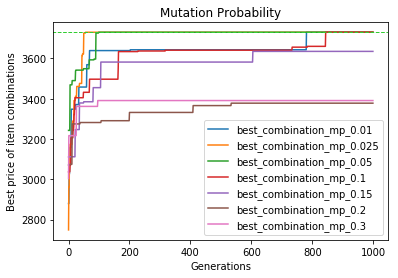
\includegraphics[height=6cm]{graphs/mutation_probability.png}
  \end{center}
  % \caption{Graf vývoje fitness}\label{fig1}
\end{figure}


\subsection{Elitismus}

Vysoký elitismus zvýhodňuje kvalitnější jedince a znevýhodňuje slabší jedince, kteří ale v sobě mohou nést lepší informaci.

Pokud toto nastavíme na vysokou hodnotu, velmi často uvízneme v lokálním maximu/minimu.

Na grafu vidíme, že elitismus se zdá být nejlepší při hodnotě 5.


\begin{figure}[H]
  \begin{center}
    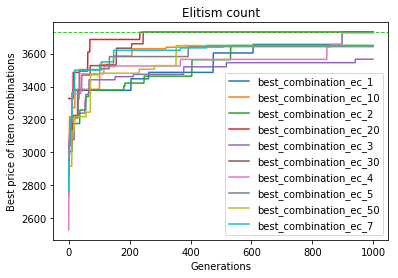
\includegraphics[height=6cm]{graphs/elitism_count.png}
  \end{center}
  % \caption{Graf vývoje fitness}\label{fig1}
\end{figure}


\subsection{Velikost turnaje}

Turnajem se vybírají jedinci ke křížení. Do každého turnaje vstupuje několik náhodných jedinců z celé populace.

Tento parametr se chová obdobně, jako elitimus, při velkých turnajích jsou znevýhodněni slabší jedinci.

Pokud toto nastavíme na vysokou hodnotu, velmi často uvízneme v lokálním maximu/minimu.

Na grafu vidíme, že velikost turnaje se zdá být nejlepší při hodnotě 2.


\begin{figure}[H]
  \begin{center}
    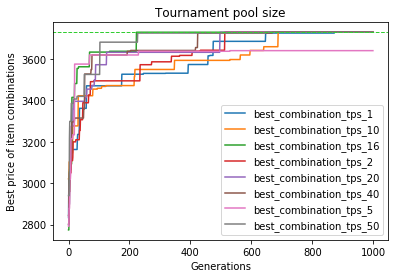
\includegraphics[height=6cm]{graphs/tournament_pool_size.png}
  \end{center}
  % \caption{Graf vývoje fitness}\label{fig1}
\end{figure}



\subsection{Počet turnajů}

Turnajem se vybírají jedinci ke křížení. Z každého turnaje je vybírán vždy jeden, tudíž počet turnajů nepřímo určuje, kolik jedinců bude vybráno ke křížení do nové populace.


Na grafu vidíme, že počet turnajů se zdá být nejlepší při hodnotě 20 až 50.



\begin{figure}[H]
  \begin{center}
    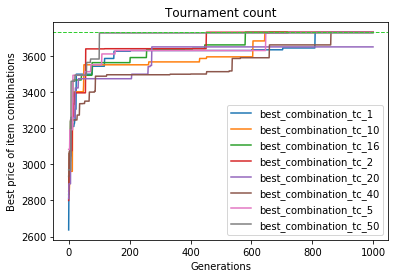
\includegraphics[height=6cm]{graphs/tournament_count.png}
  \end{center}
  % \caption{Graf vývoje fitness}\label{fig1}
\end{figure}


\subsection{Počet generací}

Počtem generací jsem zjišťoval, kolik nejméně generací je potřeba, dokud nedojde ke konvergenci, pro instance s 30 předměty.

Jako moment pro ukončení evoluce jsem vybral 1000 generací, ikdyž jak vidíme níže na grafu, tato hodnota má poměrně velkou rezervu.


\begin{figure}[H]
  \begin{center}
    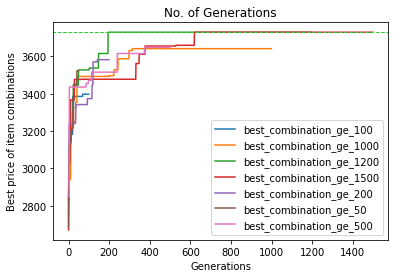
\includegraphics[height=6cm]{graphs/generations.png}
  \end{center}
  % \caption{Graf vývoje fitness}\label{fig1}
\end{figure}


\section{Výsledná konfigurace}

\begin{tabular}{l|l}
Velikost populace       & 100  \\
Počet generací          & 1000 \\
Elitismus               & 2    \\
Velikost turnaje        & 16   \\
Pravděpodobnost mutace  & 0.5  \\
Pravděpodobnost křížení & 0.5 
\end{tabular}

\section{Řešení složitějších instancí}

Jednodužší instance (tj. velikosti 40, 70, 91 klauzulí) jsou již řešeny výše.

Pro ukázku ještě vyřeším složitější instance (218 klauzulí, 50 proměnných), u kterých ale neočekávám nejlepší výsledky.


\begin{figure}[H]
  \begin{center}
    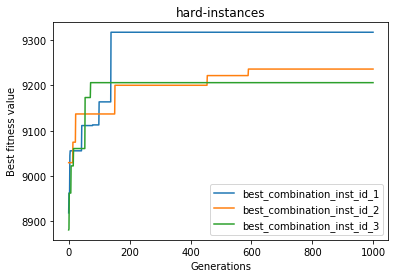
\includegraphics[height=6cm]{graphs/hard-instances.png}
  \end{center}
  % \caption{Graf vývoje fitness}\label{fig1}
\end{figure}





\\
1-hard-instances:
\\




\begin{tabular}{lrrrrrl}
\toprule
        price &  variables &  clausules &  satisfied &  weight &  valid \\
\midrule
 9317 &         50 &        218 &        210 &    1711 &  False \\
\bottomrule
\end{tabular}





\\
2-hard-instances:
\\


\begin{tabular}{lrrrrrl}
\toprule
        price &  variables &  clausules &  satisfied &  weight &  valid \\
\midrule
  9236 &         50 &        218 &        211 &     968 &  False \\
\bottomrule
\end{tabular}






\\
3-hard-instances:
\\



\begin{tabular}{lrrrrrl}
\toprule
        price &  variables &  clausules &  satisfied &  weight &  valid \\
\midrule
  9206 &         50 &        218 &        208 &    1446 &  False \\
\bottomrule
\end{tabular}

S plným úspěchem se bohužel nesetkáváme nikdy. Úspěšnost řešení měřím v procentech nalezených splněných klauzulí. Vím, že tyto instance jsou vysoce náročné a ani jsem neočekával, že bych svým algoritmem tyto instance úspěšně řešil.

Průměrně bylo dosaženo 96.6\% nalezených splněných klauzulí při 218 klauzulích na 50 proměnných (poměr 4.36, náročný).

\section{Shrnutí a závěr}

Pokročilá iterativní metoda je nesmírně (časově) efektivní při velkých počtech klauzulí a proměnných v instanci.

U instancí velikosti 40, 70 klauzulí jsme schopni nalézt optimální řešení téměř vždy napoprvé, u velikosti 91 občas je zapotřebí více běhů, ale také jsme schopni nalézt optimální řešení. 


Lehce horší je to u instancí s 218 klauzulemi, 50 proměnnými. Ale jak vidíme v předchozí kapitolce, přesnost se pohybuje nad 90\%.

Přesnost se pohybuje kolem 90-100\% (tj, relativní chyba většinou menší, než 10\%) a čas strávený výpočtem je několikařádově menší, než při použití jiných metod.

Implementace byla úspěšná a napsána pro jednoduchou výměnu batůžku  na SAT. \\
Pro vytváření grafů bylo využito Python notebooku, který je přiložen v adresáři \textbf{report/}. Grafy jsou vykresleny pomocí knihovny \textbf{mathplotlib}.

% \section{Reference}


% Tady okomentujte k čemu se váš evoluční algoritmus dopracoval, co se vám povedlo, co ne a jak by to šlo vylepšit. Jakého nejlepšího řešení se vám podařilo dosáhnout. Klidně i napište, co se vám na semestrální práci líbilo a taky co byste raději měli jinak. Uvítáme jakékoli nápady. 

% Pokud jste čerpali z nějaké literatury, měli byste ji řádně ocitovat.

% \textbf{A NEZAPOMEŇTE, ŽE SE MUSÍTE VEJÍT NA JEDNU A4! ;-)}

%%%%%%%%%%%%%%%%%%%%%%%%%%%%%%%%%%%%%%%%%%%%%%%%%%%%%%%%%%%%%%%%
% odtud dal to pak zakomentujte pomoci znaku procenta na zacatku radku
% \begin{center}
% \line(1,0){250}
% \end{center}

% \textbf{Pár poznámek pod čarou\ldots}
% \begin{itemize}
%   \item Zdroják této šablony je v kódování UTF8.
%   \item Neměňte prosím žádná nastavení dokumentu, okrajů, velikosti písma apod.
%   \item Nepřehazujte ani pořadí sekcí.
%   \item \textbf{Jak zprávu zkompilovat?} Použijte dvakrát (kvůli odkazům a referencím) tento příkaz:

%   \begin{verbatim}
%   pdflatex zdrojak-zpravy.tex
%   \end{verbatim}

%   Výsledkem bude \textbf{zdrojak-zpravy.pdf}. 

%   \item Pokud něco nepůjde, konzultujte na cvičeních BI-TED či se spolužáky. Cvičící BI-ZUM nebudou mít čas řešit detaily s {\LaTeX}em.
%   \item \textbf{Proč se sakra musím vejít na 1 A4?} Chceme, abyste si vyzkoušeli jak napsat to podstatné, vybrat to důležité, vyhnout se takové té textové vatě. Současně po vás nechceme psaní dlouhých esejí, raději svůj čas věnujte svým algoritmům. A taky, kdo má číst 5 stran napsaných \uv{protože to chtěj}. ;-)
%   \item TIP: Tuto zprávu může být reálné uplatnit i jako jeden z domácích úkolů na BI-TED. K tomu vás ale nenutíme a také počítejte s tím, že tam po vás mohou chtít další rozšíření dokumentu. \textbf{Ale zase: proč nezabít dvě mouchy jednou ranou?}
% \end{itemize}

\end{document}
